\PassOptionsToPackage{dvipsnames,svgnames,table}{xcolor}
\documentclass[11pt]{article}
\usepackage[a4paper,margin=22mm]{geometry}
\usepackage[no-math]{fontspec}
\setmainfont{DejaVu Serif}
\usepackage{amsmath,amssymb,amsthm,mathtools,graphicx,xcolor,hyperref,xurl,xspace,ifthen,enumerate}
\usepackage[shortlabels]{enumitem}
\setlength{\emergencystretch}{4em}
\AtBeginDocument{\special{pdf:mapline pzdr Dingbats <uzdr.pfb}}
\SetMathAlphabet{\mathbf}{normal}{OT1}{cmr}{bx}{n}
\SetMathAlphabet{\mathbf}{bold}{OT1}{cmr}{bx}{n}
\newtheorem{theo}{Theorem}[section]
\newtheorem{lemm}[theo]{Lemma}
\newtheorem{thm}[theo]{Theorem}
\newtheorem{proposition}[theo]{Proposition}
\newtheorem{corollary}[theo]{Corollary}
\newtheorem{definition}[theo]{Definition}
\newtheorem{theorem}[theo]{Theorem}
\newtheorem*{remas*}{Remarks}
\newtheorem{remas}[theo]{Remarks}
\newtheorem*{exam*}{Example}
\newtheorem{ques}[theo]{Question}
\providecommand{\og}{«\nobreakspace}
\providecommand{\fg}{\nobreakspace»}
\newtheorem{lem}[theo]{Lemma}
\newtheorem{lemma}[theo]{Lemma}
\newtheorem{prop}[theo]{Proposition}
\newtheorem{coro}[theo]{Corollary}
\newtheorem{corol}[theo]{Corollary}
\newtheorem*{conj*}{Conjecture}
\newtheorem{conj}[theo]{Conjecture}
\newtheorem{conjecture}[theo]{Conjecture}
\newtheorem{Proposition}[theo]{Proposition}
\newtheorem{theoreme}[theo]{Theorem}
\theoremstyle{definition}
\newtheorem{defi}[theo]{Definition}
\newtheorem{exam}[theo]{Example}
\newtheorem{exem}[theo]{Example}
\newtheorem{remark}[theo]{Remark}
\newtheorem{example}[theo]{Example}
\newtheorem{exams}[theo]{Examples}
\newtheorem{rema}[theo]{Remark}
\newtheorem{nota}[theo]{Notation}
\newtheorem{notation}[theo]{Notation}
\newtheorem*{notas}{Notations}
\newtheorem{result}[theo]{Result}
\newtheorem{question}[theo]{Question}
\newtheorem{prob}[theo]{Problem}
\newtheorem*{rema*}{Remark}
\newtheorem*{defi*}{Definition}
\newtheorem*{theo*}{Theorem}
\newtheorem*{lemm*}{Lemma}
\newtheorem*{prop*}{Proposition}
\newcommand{\enoncename}{}
\newtheorem{corpusenonce}[theo]{\enoncename}
\newenvironment{enonce}[2][]{\renewcommand{\enoncename}{#2}\begin{corpusenonce}}{\end{corpusenonce}}
\newenvironment{enonce*}[2][]{\par\medskip\noindent\textbf{#2.}\itshape}{\par\medskip}
\newenvironment{proofc}[1][\proofname]{\begin{proof}[#1]}{\end{proof}}
\newcommand{\Mc}{\mathcal{M}}
\newcommand{\pointir}{.\ ---\ }
\newcommand{\equalenv}[2]{\expandafter\let\csname#1\expandafter\endcsname\csname#2\endcsname\expandafter\let\csname end#1\expandafter\endcsname\csname end#2\endcsname}
\providecommand{\diagbox}[3][]{\begin{tikzpicture}[x=1em,y=1em,baseline=(current bounding box.center)]\useasboundingbox(0,0) rectangle(3,1.4);\draw(0,1.4)--(3,0);\node at(.5,.3){#2};\node at(2.5,1.1){#3};\end{tikzpicture}}
\providecommand{\eg}{e.g.\ }
\providecommand{\ie}{i.e.\ }
\providecommand{\cf}{cf.\ }
\providecommand{\longthanks}[1]{\par\smallskip\noindent #1\par\smallskip}
\providecommand{\qbinom}[2]{\genfrac{[}{]}{0pt}{}{#1}{#2}}

\providecommand{\mathof}[1]{\mathrm{#1}}

\numberwithin{equation}{section}


\def\endappendix{}


\usepackage{latexsym,amsmath,amssymb,verbatim,tikz,tikz-cd}
\usepackage{mathtools}
\usepackage{graphicx,xcolor}

\usepackage[english]{babel}
\usepackage{amssymb}
\usepackage{amsmath}
\usepackage{amsthm}
\usepackage{graphicx}
\usepackage{csquotes}
\usepackage{bm}
\usepackage{enumitem}
\usepackage{subcaption}
\usepackage{caption}
\renewcommand{\thesubfigure}{\Alph{subfigure}}
\usepackage{dirtytalk}
\providecommand{\nopunct}{\spacefactor1007\relax}
\newtheorem{problem}[theo]{Problem}

\newcommand{\sym}{\mathrm{Sym}}
\newcommand{\qsym}{\mathrm{QSym}}
\newcommand{\Des}{\operatorname{Des}}
\newcommand{\Asc}{\operatorname{Asc}}
\newcommand{\Syt}{\operatorname{SYT}}
\newcommand{\Short}{\operatorname{Short}}
\newcommand{\Loop}{\operatorname{Loop}}
\newcommand{\Stable}{\operatorname{Stable}}
\newcommand{\len}{\operatorname{len}}
\newcommand{\height}{\operatorname{height}}
\newcommand{\core}{\operatorname{core}}
\newcommand{\res}{\operatorname{res}}
\newcommand{\row}{\operatorname{row}}
\newcommand{\insrt}{\operatorname{insert}}
\newcommand{\UP}{\operatorname{UP}}
\newcommand{\DOWN}{\operatorname{DOWN}}


\newcommand{\ZZ}{\mathbb{Z}}
\newcommand{\NN}{\mathbb{N}}
\newcommand{\RR}{\mathbb{R}}
\newcommand{\QQ}{\mathbb{Q}}
\newcommand{\PP}{\mathbb{P}}

\newcommand{\F}{\mathcal{F}}
\newcommand{\Q}{\mathcal{Q}}
\newcommand{\A}{\mathcal{A}}
\newcommand{\M}{\mathcal{M}}
\newcommand{\I}{\mathcal{I}}
\newcommand{\PM}{\mathcal{PM}}
\newcommand{\Pcal}{\mathcal{P}}


\newcommand{\odds}{\mathrm{odds}}

\makeatletter
\newcommand{\proofstep}[1]{
  \par
  \addvspace{\medskipamount}
  \textbf{#1\@addpunct{.}}\enspace\ignorespaces
}

\newcommand\restr[2]{{
  \left.\kern-\nulldelimiterspace 
  #1 
  \vphantom{\big|} 
  \right|_{#2} 
  }}
\makeatother












\begin{document}
\section*{\raggedright 937: Sparse-statistic criterion for two-row Schur positivity of finite sets}
\noindent\textbf{Author:} Marmor, Avichai\par\noindent\textbf{Source:} Schur-positivity of short chords in matchings. Algebraic Combinatorics 7 (2024), publisher version, DOI 10.5802/alco.351. \url{https://alco.centre-mersenne.org/articles/10.5802/alco.351/}
\par\noindent\textbf{License:} CC BY 4.0, \url{https://creativecommons.org/licenses/by/4.0/}. The original publisher PDF cover has the explicit license notice. See the saved source/license records.
\par\noindent\textbf{Editorial material note (not author text):} The selected problem is original Theorem1.8 for the exact finite set and sparse statistic: both equivalence and the explicitly nonnegative two-row Schur expansion. Full author Sections1--3 preserve all three core lemmas, the complete forward proof and both original converse proofs, including sparse containment/composition symmetry and column-superstandard/conjugate-order coefficient extraction. Only two unselected numerical tableau illustrations (Figures2 and3) are omitted; the exact SYT definition, entries formula, formal column-superstandard construction and every proof remain editable unchanged. Their incidental references keep original printed figure numbers. The later matching bijections/refinements are unselected and preserve printed source pointers. No tableau, proof, positivity argument or formula is reconstructed. The author original ytableau/shuffle/youngtab/bbm/accents imports are genuinely unused throughout this retained body after the two ancillary illustration omissions; no tableau or shuffle glyph substitution is used. All proof text and formulas below are editable author TeX. Mathematical wording, language and proof order are retained. Only the article class, title matter and bibliography presentation are adapted for independent compilation; no proof has been generated or repaired.
\par\noindent\textbf{Editorial difficulty:} H2: The converse reconstructs symmetry from sparse containment counts and isolates Schur coefficients using column-superstandard tableaux and conjugate-order maximality. The full symmetry-forcing and coefficient-positivity argument is retained, not merely the resulting matching enumeration or a direct Pieri expansion.
\medskip\hrule\medskip
\noindent\textbf{Author statement, complete proof and local supporting text follow in source order.}
\section{Introduction}
\label{sec:introduction}

Denote the set of nonnegative integers by $\NN$, and the set of positive integers by $\PP$. Given $N\in \NN$ and a set $\A$, together with a set-valued function $D:\A\to 2^{[N-1]}$ which is sometimes called a \emph{statistic}, we define its quasisymmetric generating function
\[
    \Q_{D} (\A) = \sum_{a \in \A} F_{N, D(a)},
\]
where $F_{N, S}$ is the \emph{fundamental quasisymmetric function} introduced by Gessel~\cite{knuth_classes_schur_positive}, indexed by a subset $S \subseteq [N-1]$ (see Section~\ref{subsec:definitions symmetric functions} for more background). We write $\Q(\A)$ instead of $\Q_{D}(\A)$ when $D$ is clear from the context.
The following long-standing problem was first addressed in~\cite{gessel1993counting}.
\begin{problem}[Gessel and Reutenauer]
    Find sets $\A$ and statistics $D$ for which $\Q_{D}(\A)$ is symmetric.
\end{problem}

When $\Q_{D}(\A)$ is symmetric, we say that $\A$ is symmetric with respect to the statistic $D$ (we omit $D$ when it is clear from the context). If $\A$ is symmetric, then there is a unique expansion
\[
    \Q_{D} (\A) = \sum_{\lambda \vdash N} c_\lambda s_\lambda,
\]
where $c_\lambda \in \QQ$ and $s_\lambda$ are Schur functions (discussed in Section~\ref{subsec:definitions symmetric functions}). The coefficients $c_\lambda$ are called the \emph{Schur coefficients} of $\A$.
If $c_\lambda \in \NN$ for all $\lambda \vdash N$, we say that $\A$ is Schur-positive with respect to $D$.

Gessel and Reutenauer also addressed the following problem:
\begin{problem}
    Find Schur-positive sets $\A$.
\end{problem}






The study of symmetric functions is partially motivated by the correspondence between symmetric functions of degree $N$ and class functions on the symmetric group $S_N$, which is established through the Frobenius characteristic map described in~\cite[Chapter 4.7]{sagan_book}. A symmetric function is Schur-positive if its corresponding class function is a proper character (see~\cite{adin_roichman_fine_set} for a detailed explanation). This perspective provides a rich algebraic framework for studying symmetric and Schur-positive sets.

During the last few decades, many Schur-positive subsets of the symmetric group $S_N$ were constructed with respect to the standard descent function of $S_N$, where a permutation $\pi \in S_N$ has $i \in \Des(\pi)$ if and only if $\pi(i) > \pi(i+1)$. A fundamental construction is due to Gessel~\cite{knuth_classes_schur_positive}, who proved that every set of permutations which is closed under the Knuth equivalence relations is Schur-positive. Furthermore, he showed that every Knuth class $\A \subset S_N$ (\ie equivalence class of the Knuth relations) satisfies $\Q_{\Des}(\A) = s_\lambda$ for some $\lambda \vdash N$. This result has many direct consequences. For example, for every $J \subseteq [N-1]$, the set $D_{N,J}^{-1} = \{ \pi^{-1} \mid \Des(\pi)=J\} \subseteq S_N$ is Schur-positive because it is closed under the Knuth relations.

Other examples of Schur-positive sets of permutations include all conjugacy classes, as proven by Gessel and Reutenauer~\cite{gessel1993counting}, and the set of permutations $\pi \in S_N$ with a fixed number of inversions (\ie $i<j$ such that $\pi(i) > \pi(j)$), a result demonstrated by Adin and Roichman \cite[Prop.\ 9.5]{adin_roichman_fine_set}.

Some Schur-positive sets that do not consist of permutations were found as well. For instance, Gessel~\cite{knuth_classes_schur_positive} proved that for every partition $\lambda \vdash N$, the set $\Syt(\lambda)$ of standard Young tableaux of shape $\lambda$ is Schur-positive (see Section~\ref{subsec:schur positive sets} for details).

In this work, we focus on the set of matchings of a given set of vertices.
\begin{definition}
\label{def:matching}
    A matching $m$ on a finite set of vertices $S \subseteq \PP$ is an unordered partition of $S$ into blocks, each block of size $1$ or $2$. If a block of a matching $m$ contains only the vertex $i$, we say that $i$ is an \emph{unmatched vertex} of $m$ and denote $(i) \in m$. If a block contains both $i$ and $j$ for $i<j$, we say that $(i,j)$ is a \emph{chord} of $m$ and denote $(i,j) \in m$. That is, the notation $(i,j)\in m$ implies that $i<j$. When $(i,j) \in m$, we also say that $i$ opens this chord and $j$ closes it. If a matching $m$ has no unmatched vertex, then we say that $m$ is a perfect matching.
\end{definition}

We will focus on matchings on the set $[N] := \{1,\dots, N\}$ for some $N \in \NN$. Denote by $\M_N$ the set of matchings on $[N]$, and by $\M_{N,f}$ the set of matchings on $[N]$ with $f$ unmatched vertices.

For example, 
\[
    \M_{4,0} = \big\{\{(1,2),\; (3,4)\},\ \{(1,3),\; (2,4)\},\ \{(1,4),\; (2,3)\}\big\}
\]
and
\[ 
    \M_{3,1} = \big\{\{(1,2),\; (3)\},\ \{(1,3),\; (2)\},\ \{(1),\; (2,3)\}\big\}.
\]

\begin{definition}
\label{def:intersect}
    Let $m$ be a matching on $S$. If $(i_1, i_3),\: (i_2,i_4) \in m$ for $i_1 < i_2 < i_3 < i_4$ then we say that the chords $(i_1, i_3)$ and $(i_2, i_4)$ \emph{intersect}.
\end{definition}

\begin{definition}
\label{def:short}
    Let $m \in \M_N$ be a matching on $[N]$. If $(i,i+1) \in m$, then it is called a \emph{short chord}. We denote $\Short(m) := \{i \in [N-1] \mid (i,i+1) \in m\}$.

\end{definition}

For example, consider the matching $m = \{(1,3),\; (2,6),\; (4,5)\}$ as in Figure~\ref{fig:matching example introduction}. In this matching the chords $(1,3)$ and $(2,6)$ intersect, and $\Short(m) = \{4\}$ (since $(4,5) \in m$).
\begin{figure}[htb]
    \begin{center}
        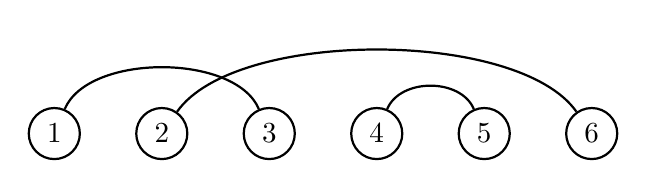
\begin{tikzpicture}[node distance={13mm}, thick, main/.style = {draw, circle, scale=1.05}]  
            \node[main] (1) {$1$};
            \node[main] (2) [right of=1] {$2$};
            \node[main] (3) [right of=2] {$3$};
            \node[main] (4) [right of=3] {$4$};
            \node[main] (5) [right of=4] {$5$};
            \node[main] (6) [right of=5] {$6$};
            
            
            \draw (1) to [out=67,in=113,looseness=0.8] (3);
            \draw (2) to [out=55,in=125,looseness=0.65] (6);
            \draw (4) to [out=67,in=113,looseness=1] (5);
        \end{tikzpicture}
    \end{center}
    \caption{The matching $m = \{(1,3),\; (2,6),\; (4,5)\}$.}
    \label{fig:matching example introduction}
\end{figure}

Note that $N \notin \Short(m)$ for every $m \in \M_N$. This holds even where $(1,N) \in m$.



Enumerative properties of short chords in perfect matchings were studied extensively. The distribution of the number of short chords in perfect matchings appears in entry A079267 of the OEIS~\cite{oeis}, and was analyzed for example by Cameron and Killpatrick~\cite{killpatrick2020statistics}. McSorley and Feinsilver~\cite{bessel_polynomials_mathcings} discovered that short chords of matchings are closely related to Bessel polynomials, as will be discussed in Section~4.3.

The study of short chords of matchings is also motivated by the involutive length and its corresponding poset studied by Adin, Postnikov and Roichman~\cite{gelfand_involutions}. Related posets derived from the Bruhat order were studied by Richardson and Springer~\cite{richardson1990bruhat}, Hultman~\cite{hultman2008twisted}, Deodhar and Srinivasan~\cite{deodhar2001statistic} and others, motivated by the topology of linear algebraic groups (see~\cite{hultman2008twisted} for details). Further discussion on the algebraic motivations can be found in Section~6.3.




We prove the following:
\begin{theorem}
\label{thm:matchings schur positive}
    Let $n,f \in \NN$ be nonnegative integers, and denote $N=2n+f$. Then the set $\M_{N,f}$ is Schur-positive with respect to $\Short$. Furthermore, its Schur expansion is given by the following formula:
    \[
        \Q_{\Short} (\M_{N,f}) = \sum_{k=0}^n |\{ m\in \M_{N-2k,f} \mid \Short(m) = \emptyset\}|\ s_{N-k,k}.
    \]
\end{theorem}

It turns out  that the Schur coefficients of $\Q_{\Short} (\M_{N,f})$ 
may be explicitly interpreted in terms of Bessel polynomials, see 
Corollary~4.13 
below.




We give two proofs of Theorem~\ref{thm:matchings schur positive}. The first proof relies on a new criterion for Schur-positivity of sparse statistics:

\begin{definition}
\label{def:sparse}
    We say that a set $J \subseteq [N-1]$ is \emph{sparse} if $\{j,j+1\} \nsubseteq J$ for every $1 \le j \le N-2$.

    For a set $\A$ and a function $D:\A \to 2^{[N-1]}$, we say that $D$ is \emph{sparse} if $D(a)$ is sparse for all $a \in \A$.
\end{definition}

\begin{theorem}
\label{thm:criterion schur positive two rows}
    Let $\A$ be a finite set with a statistic $D:\A \to 2^{[N-1]}$, and denote $n = \lfloor\frac{N}{2} \rfloor$. Then the following statements are equivalent:
    \begin{itemize}
        \item $D$ is sparse, and for every sparse $J \subseteq [N-1]$, the cardinality of the set $\{a \in \A \mid D(a) \supseteq J\}$ depends on the size of $J$ only.
        \item $\A$ is symmetric with respect to $D$, with a Schur expansion of the form $\Q_{D}(\A) = \sum_{k=0}^n c_k s_{N-k,k}$ for some $c_k \in \ZZ$.
    \end{itemize}

    Furthermore, if these statements hold then $\A$ is Schur-positive, and its Schur expansion is
    \[
        \Q_{D} (\A) = \sum_{k=0}^n \left|\left\{ a\in \A \mid D(a) = \{1,3,5,\dots, 2k-1\} \right\}\right|\: s_{N-k,k}.
    \]
    
\end{theorem}

This new criterion implies Theorem~\ref{thm:matchings schur positive}, %
as shown at the beginning of Section~4, and can be applied to many other sets as well.
It is also applied in a subsequent paper \cite{gallai} to prove Schur-positivity of Gallai colorings and transitive colorings of complete graphs.

The second proof of Theorem~\ref{thm:matchings schur positive} provides a bijection from the set of matchings to a multiset of SYTs,
and applies the bijective criterion of Adin and Roichman for Schur-positivity \cite[Prop.\ 9.1]{adin_roichman_fine_set}, presented in Theorem~\ref{thm:criterion schur positive young}.

Following the bijective proof, we present an equivalence relation on matchings, motivated by Knuth equivalence of permutations~\cite{knuth1970permutations}:
\begin{definition}\label{def:knuth like equivalence}
    We say that two matchings $m_1,m_2 \in \M_N$ are \emph{Knuth equivalent} if one can be obtained from the other by a sequence of \emph{elementary Knuth transformations}:
    \begin{itemize}
        \item Replace the chords $(i,i+1),\; (i+2)$ with the chords $(i),\; (i+1,i+2)$ or vice versa (\ie interchange a short chord with an adjacent unmatched vertex).
        \item Replace the chords $(i,i+1),\; (i+2,j)$ with the chords $(i,j),\; (i+1,i+2)$, or $(i,i+1),\; (j,i+2)$ with $(j,i),\; (i+1,i+2)$, or vice versa (\ie interchange a short chord with an adjacent endpoint of another chord).
    \end{itemize}
\end{definition}

We also define the core of a given matching:

\begin{definition}[Definition~4.3 below]
    The \emph{core} of a given matching $m \in \M_N$, denoted $\core(m)$, is obtained by repeatedly removing short chords from the matching until no short chords remain. The remaining vertices are then re-indexed with natural numbers starting from $1$ while preserving their relative order.

\end{definition}

A classical result due to Knuth~\cite{knuth1970permutations} states that two permutations $\pi_1,\pi_2 \in S_N$ are Knuth equivalent if and only if $P(\pi_1) = P(\pi_2)$, where $P(\pi)$ denotes the insertion tableau of a permutation $\pi$ defined by the Robinson-Schensted correspondence (see \cite[Section 3]{sagan_book} for details). We prove the following analogous result for matchings:
\begin{theorem}[Theorem~5.1 below]
    Two matchings $m_1, m_2 \in \M_N$ are Knuth equivalent if and only if $\core(m_1) = \core(m_2)$.
\end{theorem}

We show that Knuth classes of matchings, similarly to Knuth classes of permutations, have Schur functions as their generating functions:

\begin{theorem}[Corollary~5.9 below]
    Every set $\M \subseteq \M_N$ of matchings that is closed under Knuth equivalence is Schur-positive with respect to $\Short$. Moreover, if $\M$ is a Knuth equivalence class, then its generating function is $\Q_{\Short}(\M) = s_{N-k,k}$, where $N-2k$ is the number of vertices of $\core(m)$ for some arbitrary matching $m \in \M$.
\end{theorem}

Furthermore, utilizing Knuth classes, we explore in Section~5 various refined Schur-positive sets, including:
\begin{itemize}
    \item The set of $k$-crossing matchings (\ie where $k$ is the maximal cardinality of a set of pairwise intersecting chords).
    \item The set of matchings with exactly $k$ pairs of intersecting chords.
\end{itemize}

Lastly, we define $\M_{N,f}(m)$ as the set of matchings in $\M_{N,f}$ that avoid the pattern $m$. In Proposition~5.14, we provide a characterization of the matchings $m$ for which $\M_{N,f}(m)$ is Schur-positive for all $N$ and $f$.

The remainder of this work is organized as follows: Section~\ref{sec:preliminaries} provides necessary background. In Section~\ref{sec:criterion two rows}, we prove a necessary and sufficient criterion for sparse Schur-positivity (Theorem~\ref{thm:criterion schur positive two rows}). In Section~4, we focus on matchings. We first derive the Schur-positivity of short chords in matchings (Theorem~\ref{thm:matchings schur positive}) from the above criterion. Then, we present an alternative bijective proof, followed by a description of the Schur coefficients of matchings in terms of Bessel polynomials. In Section~5, we utilize the bijection to refine the Schur-positivity property of Theorem~\ref{thm:matchings schur positive}. Finally, Section~6 concludes with further remarks and open problems.

\section{Preliminaries and notation}
\label{sec:preliminaries}

\begin{definition}
    For nonnegative integers $i,j$, we define the \emph{interval}
    \[
        [i,j] :=
        \begin{cases}
            \{i,i+1,\dots,j\} & \text{if $i \le j$,}\\
            \emptyset & \text{otherwise.}
        \end{cases}
    \]
    We also define $[i] = [1,i]$.
\end{definition}

\begin{definition}
\label{def:elements with given stat}
    Given a set $\A$, a function $D:\A \to 2^{[N-1]}$ and a set $J \subseteq [N-1]$, we denote $\A(D=J) := \{a \in \A \mid D(a) = J\}$ and $\A(D \supseteq J) := \{a \in \A \mid D(a) \supseteq J\}$.
\end{definition}

\subsection{Symmetric and quasisymmetric functions}
\label{subsec:definitions symmetric functions}

\begin{definition}
    Given $N \in \NN$, a \emph{partition} $\lambda$ of $N$ (denoted $\lambda \vdash N$), is a weakly-decreasing sequence $\lambda = (\lambda_1 \ge \lambda_2 \ge \dots \ge \lambda_\ell)$ of positive integers, such that $\lambda_1 + \dots + \lambda_\ell = N$. The values $(\lambda_1,\dots,\lambda_\ell)$ are called the \emph{parts} of $\lambda$.
    
    A \emph{composition} $\alpha$ of $N$ (denoted $\alpha \vDash N$) is a sequence $\alpha = (\alpha_1, \alpha_2, \dots, \alpha_\ell )$ of positive integers, such that $\alpha_1 + \dots + \alpha_\ell = N$. Every partition is a composition.
\end{definition}

Compositions of $N$ are in bijection with subsets of $[N-1] := \{1, \dots, N-1\}$ by 
\[
    [N-1] \supseteq \{i_1, i_2, \dots, i_\ell \} \mapsto (i_1, i_2 - i_1, \dots, i_\ell - i_{\ell-1}, N - i_\ell) \vDash N.
\]
For example, for $N = 10$, $\{2, 4, 7, 8\} \mapsto (2, 2, 3, 1, 2)$. The composition associated to a set $S$ is denoted $\alpha_S$, and the set associated to a composition $\alpha$ is denoted $S_\alpha$.

We say that two compositions $\alpha, \beta \vDash N$ are \emph{equivalent} (denoted $\alpha \sim \beta$), if $\beta$ is a rearrangement of the entries of $\alpha$.

Denote the ring of symmetric functions by $\sym$ and the ring of quasisymmetric functions by $\qsym$ (see, for example, \cite[Section 1]{S3_patterns_list} for details). The space of homogeneous symmetric functions of degree $N$ is denoted by $\sym_N$, and the space of homogeneous quasisymmetric functions of degree $N$ is denoted by $\qsym_N$.

The space $\qsym_N$ has several important bases. In this work, we focus on the \emph{fundamental basis}, consisting of the functions
\[
    F_{N,S} := \sum_{\substack{i_1 \le i_2 \le \dots \le i_N \\ \forall j \in S:i_j < i_{j+1}}} x_{i_1} x_{i_2} \dots x_{i_N},\quad S \subseteq [N - 1].
\]
We write $F_S$ instead of $F_{N,S}$ when $N$ is clear from the context.

The space $\sym_N$ has several standard bases as well. In this work, we focus on the Schur basis, which consists of the Schur functions $s_{\lambda}$, where $\lambda$ is a partition of $N$. 
The definition and properties of Schur functions can be found in \cite[Section 4.4]{sagan_book}. Here, we adopt the combinatorial approach to Schur functions, as described in Theorem~\ref{thm:schur functions young tableaux} and Theorem~\ref{thm:criterion schur positive young} below.

\subsection{Symmetric and Schur-positive sets}
\label{subsec:schur positive sets}
As mentioned in Section~\ref{sec:introduction}, a set $\A$ is symmetric with respect to a statistic $D:\A \to 2^{[N-1]}$ if the generating function $\Q_{D}(\A)$ is a symmetric function. Moreover, it is Schur-positive if all Schur coefficients are nonnegative integers.


One of the fundamental constructions of Schur-positive sets, regarding sets of standard Young tableaux (SYT), is due to Gessel~\cite{knuth_classes_schur_positive}. Let $\Syt(\lambda)$ denote the set of standard Young tableaux of shape $\lambda$. We draw tableaux in English notation, as in Figure~2. The \emph{descent set} of $T\in \Syt(\lambda)$ is
\[
    \Des(T) := \{i \in [N-1] \mid i+1 \text{ appears in a lower row than $i$ in $T$}\}.
\]
For example, the descent set of the SYT in Figure~2 is $\{2,4,7,8\}$.

The entry in row $i$ and column $j$ of a tableau $T \in \Syt(\lambda)$ is denoted by $T_{i,j}$. In addition, we define $\row_i(T) := \{T_{i,j} \mid 1 \le j \le \lambda_i\}$ as the set of entries in the $i$-th row of $T$. For example, if we consider the SYT shown in Figure~2, then $T_{3,2} = 8$ and $\row_3(T) = \{5,8\}$.

\begin{theorem}[Gessel~\cite{knuth_classes_schur_positive}]
\label{thm:schur functions young tableaux}
    For every $\lambda \vdash N$, the set $\Syt(\lambda)$ is Schur-positive with respect to $\Des$. Moreover, $\Q(\Syt(\lambda)) = s_\lambda$.
\end{theorem}

In 2015, Adin and Roichman proved the following criterion.
\begin{theorem}[{\cite[Prop.\ 9.1]{adin_roichman_fine_set}}]
\label{thm:criterion schur positive young}
    A set $\A$ is symmetric with respect to $D:\A\to 2^{[N-1]}$ if and only if
    \[
        \sum_{a \in \A} \boldsymbol{t}^{D(a)} = \sum_{\lambda \vdash N} c_\lambda \sum_{T \in \Syt(\lambda)} \boldsymbol{t}^{\Des(T)}
    \]
    for some values $c_\lambda$, where $\boldsymbol{t}^J := \prod_{j \in J} t_j$ for $J \subseteq [N-1]$. The coefficients $c_\lambda$ are the Schur-coefficients of $\A$. Moreover, $\A$ is Schur-positive if and only if $c_{\lambda} \in \NN$ for all $\lambda \vdash N$.
\end{theorem}

This criterion implies that proving the Schur-positivity of a set is achievable by establishing a statistic-preserving bijection between the set and SYTs of shapes corresponding to a specific multiset.

In this paper, we will also apply a recently formulated criterion for symmetry~\cite{my_pattern_theorem}.
\begin{definition}
\label{def:respect composition}
    Let $\A$ be a finite set with a statistic $D:\A \to 2^{[N-1]}$. The set of elements that \emph{respect} a given composition $\alpha \vDash N$, denoted $\A_D(\alpha)$, consists of the elements $a \in \A$ such that $D(a) \subseteq S_\alpha$, where $S_\alpha$ is the set corresponding to the composition $\alpha$. When $D$ is clear from the context, we may write $\A(\alpha)$ instead.
\end{definition}

\begin{lemma}
\label{lem:my symmetry criterion}
    A set $\A$ is symmetric if and only if $|\A(\alpha)| = |\A(\beta)|$ for all $\alpha \sim \beta \vDash N$.
\end{lemma}

Note that only sets of permutations are considered in~\cite{my_pattern_theorem}. However, Lemma~\ref{lem:my symmetry criterion} applies to other sets as well.



    

    

Another useful result about symmetric sets and symmetric functions is due to Bloom and Sagan:
\begin{lemma}[Bloom and Sagan {\cite[Lemma 2.2]{BloomSagan}}]
\label{lem:singleton not symmetric}
    
    For every set $S \subseteq [N-1]$, the function $F_{N,S}$ is symmetric if and only if $S=[N-1]$ or $S=\emptyset$.
\end{lemma}


\section{Proof of Theorem~\ref{thm:criterion schur positive two rows}}
\label{sec:criterion two rows}

Denote $\odds(k) := \{1,3,5,\dots, 2k-1\}$ for a nonnegative integer $k$. In particular, $\odds(0) = \emptyset$.

Recall Definition~\ref{def:sparse} and Definition~\ref{def:elements with given stat}. We divide the assertions of Theorem~\ref{thm:criterion schur positive two rows} into two propositions:
\begin{lemma}
\label{lem:if schur positive two rows then sparse and good sizes}
    Let $\A$ be a symmetric set with respect to a statistic $D:\A \to 2^{[N-1]}$, and denote $n = \lfloor\frac{N}{2} \rfloor$. Assume that the Schur expansion of $\A$ is $\Q_{D}(\A) = \sum_{k=0}^n c_k s_{N-k,k}$ for some $c_k \in \ZZ$. Then
    $D$ is a sparse function, and for every sparse set $J \subseteq [N-1]$, the cardinality of the set $\A(D \supseteq J)$ depends on the size of $J$ only.
\end{lemma}
\begin{lemma}
\label{lem:if sparse and good sizes then schur positive two rows}
    Let $\A$ be a finite set with a sparse statistic $D:\A \to 2^{[N-1]}$, and denote $n = \lfloor\frac{N}{2} \rfloor$. Assume that for every sparse set $J \subseteq [N-1]$, the cardinality of the set $\A(D \supseteq J)$ depends on the size of $J$ only.
    Then $\A$ is Schur-positive, and its Schur expansion is
    \[
        \Q_{D} (\A) = \sum_{k=0}^n |\A(D=\odds(k))|\; s_{N-k,k}.
    \]
\end{lemma}

We prove Lemma~\ref{lem:if schur positive two rows then sparse and good sizes} in Section~\ref{subsec:proof lemma if schur positive two rows then sparse and good sizes}, and then show two proofs for Lemma~\ref{lem:if sparse and good sizes then schur positive two rows}. The first proof (presented in Section~\ref{subsec:proof if sparse and good sizes then schur positive two rows by induction}) is inductive. The second proof (presented in Section~\ref{subsec:proof if sparse and good sizes then schur positive two rows by superstandard}) is more involved, and it demonstrates the power of column superstandard tableaux, introduced by Hamaker, Pawlowski and Sagan~\cite{S3_patterns_list}, in proving Schur-positivity properties. We believe this approach can be applied in other cases as well.

Before proving these lemmas, let us prove a simple folklore lemma that will be useful for both lemmas:
\begin{lemma}
\label{lem:symmetric complement is symmetric}
    Let $\A$ be a symmetric set with respect to a statistic $D:\A \to 2^{[N-1]}$. Then $\A$ is also symmetric with respect to the complementary statistic $\bar{D}:\A \to 2^{[N-1]}$ defined by $a \mapsto [N-1]\setminus D(a)$.
\end{lemma}
\begin{proof}
    The set $\A$ is symmetric with respect to $D$, so by Theorem~\ref{thm:criterion schur positive young} there exist values $c_{\lambda},\ \lambda \vdash N$ such that
    \[
        \sum_{a \in \A} \boldsymbol{t}^{D(a)} = \sum_{\lambda \vdash N} c_\lambda \sum_{T \in \Syt(\lambda)} \boldsymbol{t}^{\Des(T)},
    \]
    where $\boldsymbol{t}^J := \prod_{j \in J} t_j$ for $J \subseteq [N-1]$, and therefore
    \[
        \sum_{a \in \A} \boldsymbol{t}^{[N-1]\setminus D(a)} = \sum_{\lambda \vdash N} c_\lambda \sum_{T \in \Syt(\lambda)} \boldsymbol{t}^{[N-1]\setminus \Des(T)} = \sum_{\lambda \vdash N} c_\lambda \sum_{T \in \Syt(\lambda')} \boldsymbol{t}^{\Des(T)},
    \]
    where $\lambda'$ is the partition conjugate to $\lambda$.
\end{proof}

\subsection{Proof of Lemma~\ref{lem:if schur positive two rows then sparse and good sizes}}
\label{subsec:proof lemma if schur positive two rows then sparse and good sizes}
\begin{proof}[\unskip\nopunct]
    The set $\A$ is symmetric, and its Schur expansion is $\Q_{D}(\A) = \sum_{k=0}^n c_k s_{N-k,k}$. Therefore, by Theorem~\ref{thm:criterion schur positive young}, we have
    \begin{equation}\label{eqn:proof if schur positive two rows then sparse}
        \sum_{a \in \A} \boldsymbol{t}^{D(a)} = \sum_{k=0}^n c_k \sum_{T \in \Syt(N-k,k)} \boldsymbol{t}^{\Des(T)}.
    \end{equation}
    First of all, notice that the set $\Des(T)$ is sparse for all $T \in \Syt(N-k,k)$. Therefore, by Equation~\eqref{eqn:proof if schur positive two rows then sparse}, the set $D(a)$ is sparse for all $a \in \A$.
    
    It remains to show that for every sparse set $J \subseteq [N-1]$ of size $k$, we have $\left|\A(D \supseteq J)\right| = \left|\A(D \supseteq \odds(k))\right|$. Denote $\alpha = (2^k,1^{N-2k}) \vDash N$. Additionally, let $i_1 < \dots < i_{N-k-1} \in [N-1]\setminus J$ denote the elements not in $J$. Since $J$ is sparse, the differences $i_{t+1} - i_t$ for $1 \le t \le N-k-2$, as well as $i_1$ and $N - i_{N-k-1}$, are either 1 or 2. Those that are equal to 2 correspond to the elements of $J$. The composition associated to the set $[N-1]\setminus J$ is denoted by $\beta := (i_1, i_2 - i_1, i_3 -i_2, \dots, i_{N-k-1} - i_{N-k-2}, N-i_{N-k-1}) \vDash N$. By Lemma~\ref{lem:symmetric complement is symmetric}, $\A$ is symmetric with respect to the complementary statistic $\bar{D}$. Notably, the compositions $\alpha$ and $\beta$ are equivalent, as they both have $k$ occurrences of $2$ and $N-2k$ occurrences of $1$. By Lemma~\ref{lem:my symmetry criterion}, we obtain that $|\A_{\bar{D}}(\beta)| = |\A_{\bar{D}}(\alpha)|$. By Definition~\ref{def:respect composition}, we obtain that $\A_{\bar{D}}(\beta) = \A(D \supseteq J)$ and $\A_{\bar{D}}(\alpha) = \A(D \supseteq \odds(k))$. Consequently, $|\A(D \supseteq J)| = |\A(D \supseteq \odds(k))|$, as required.
\end{proof}

\subsection{First proof of Lemma~\ref{lem:if sparse and good sizes then schur positive two rows}}
\label{subsec:proof if sparse and good sizes then schur positive two rows by induction}
We start by introducing an observation, which will serve as a crucial step in our inductive argument.
\begin{lemma}
\label{lem:remove first descent from syt}
    Let $k_1 \ge k_2$ be two nonnegative integers, and let $J \subseteq [k_1 + k_2 - 1]$ be a set. Then
    \[
        \left|\Syt(k_1, k_2)(\Des \supseteq J)\right| = \left|\Syt\big(k_1+1, k_2+1\big)\big(\Des \supseteq (\{1\}\cup (J+2))\big)\right|,
    \]
    where $J+2 = \{j + 2 \mid j \in J\}$.
\end{lemma}
\begin{proof}
    The proof is bijective: We associate a given tableau $T \in \Syt(k_1, k_2)$ such that $\Des(T) \supseteq J$ with the tableau $T' \in \Syt(k_1+1, k_2+1)$ defined by $T'_{1,1} = 1,\; T'_{2,1} = 2$, and for all $i \in \{1,2\}$ and $j \in [k_i]$, $T'_{i,j+1} = T_{i,j}+2$ (recall that $T_{i,j}$ is the entry in row $i$ and column $j$ of $T$). Intuitively, we first increase every entry of $T$ by $2$. Then, we insert a new column with the letters $1,2$ on the left of $T$, shifting the other columns to the right. Clearly, this process is injective, and $T'$ satisfies $T' \in \Syt(k_1+1, k_2+1)$ and $\Des(T) \supseteq \{1\}\cup (J+2)$. Furthermore, any $T' \in \Syt(k_1+1, k_2+1)$ with $\Des(T') \supseteq \{1\}\cup (J+2)$ can be obtained through this process.
\end{proof}

Now we are ready to prove Lemma~\ref{lem:if sparse and good sizes then schur positive two rows}.
\begin{proof}[First proof of Lemma~\ref{lem:if sparse and good sizes then schur positive two rows}]
    Let $\A$ be a finite set with a sparse statistic $D:\A \to 2^{[N-1]}$, and assume that for every sparse set $J \subseteq [N-1]$, the cardinality of the set $\A(D \supseteq J)$ depends on the size of $J$ only.
    By Theorem~\ref{thm:criterion schur positive young}, it suffices to show that
    \begin{equation}\label{eqn:first proof no consecutive indices is schur positive - generating function}
        \sum_{a \in \A} \boldsymbol{t}^{D(a)} = \sum_{k=0}^n |\A(D=\odds(k))| \sum_{T \in \Syt(N-k,k)} \boldsymbol{t}^{\Des(T)},
    \end{equation}
    where $n = \lfloor\frac{N}{2}\rfloor$.
    
    We prove it by induction on $N \in \NN$:
    
    For $N \le 1$, the statement holds trivially.
    
    Next, we assume that the statement holds for every value smaller than $N$ and proceed to prove it for $N$. Our goal is to establish the equation:
    \begin{equation}\label{eqn:first proof no consecutive indices is schur positive - set equality}
        \left|\A(D=J)\right| = \sum_{k=0}^n c_k \left|\Syt(N-k,k)(\Des=J)\right|
    \end{equation}
    for every set $J \subseteq [N-1]$, where $c_k = \left|\A(D=\odds(k))\right|$.
    
    We begin by considering the case $J = \emptyset$. In this case, the only SYT $T$ with $\Des(T) = \emptyset$ is the unique tableau of one row. Consequently, Equation~\eqref{eqn:first proof no consecutive indices is schur positive - set equality} simplifies to $\left|\A(D=\emptyset)\right| = \left|\A(D=\odds(0))\right|$, which obviously holds.
    
    It now remains to prove Equation~\eqref{eqn:first proof no consecutive indices is schur positive - set equality} for all $J \ne \emptyset$. By  the inclusion--exclusion principle, it suffices to prove that the following holds for all $J \ne \emptyset$:
    \begin{equation}\label{eqn:first proof no consecutive indices is schur positive - set containment}
        \left|\A(D \supseteq J)\right| = \sum_{k=0}^n c_k \left|\Syt(N-k,k)(\Des \supseteq J)\right|.
    \end{equation}
    
    The function $D$ is assumed to be sparse, and the set $\Des(T)$ is sparse for all $T \in \Syt(N-k,k)$. Therefore, if $J$ is not sparse then Equation~\eqref{eqn:first proof no consecutive indices is schur positive - set containment} holds.

    Next, let $J \ne \emptyset$ be a sparse set, and denote $|J| = i$. The set $\odds(i)$ is sparse too, and has $i$ elements. Therefore, by the assumptions of the lemma, we obtain that $\left|\A(D \supseteq J)\right| = \left|\A(D \supseteq \odds(i))\right|$.
    In addition, by Theorem~\ref{thm:schur functions young tableaux}, the set $\Syt(N-k,k)$ is Schur-positive and has the Schur expansion $\Q(\Syt(N-k,k)) = s_{N-k,k}$. Therefore, we can apply Lemma~\ref{lem:if schur positive two rows then sparse and good sizes} and deduce that
    \[
        \left|\Syt(N-k,k)(\Des \supseteq J)\right| = \left|\Syt(N-k,k)(\Des \supseteq \odds(i))\right|.
    \]
    Therefore, Equation~\ref{eqn:first proof no consecutive indices is schur positive - set containment} reduces to
    \begin{equation}\label{eqn:first proof no consecutive indices is schur positive - odds set}
        \left|\A(D \supseteq \odds(i))\right| = \sum_{k=0}^n c_k \left|\Syt(N-k,k)(\Des \supseteq \odds(i))\right|,
    \end{equation}
    where $i > 0$. Thus, the proof will be completed when we establish Equation~\eqref{eqn:first proof no consecutive indices is schur positive - odds set}.
    
    Denote $\A_1 = \{a \in \A \mid 1\in D(a)\}$. Furthermore, define a new statistic $D_1:\A_1 \to 2^{[N-3]}$ by $D_1(a) = (D(a)\setminus\{1\})-2$. Notice that $\A_1$ satisfies the requirements of Lemma~\ref{lem:if sparse and good sizes then schur positive two rows} with respect to $D_1$, where $N$ is replaced by $N-2$. Therefore, we may assume, by the induction hypothesis, that Lemma~\ref{lem:if sparse and good sizes then schur positive two rows} holds for $\A_1$. Thus, we can apply Equation~\eqref{eqn:first proof no consecutive indices is schur positive - set containment} for $\A_1$, while replacing $c_k$ with $|\A_1(D_1 = \odds(k))| = |\A(D = \odds(k+1))| = c_{k+1}$, and obtain
    \begin{equation}\label{eqn:first proof no consecutive indices is schur positive - induction}
        \left|\A_1(D_1 \supseteq J)\right| = \sum_{k=0}^{n-1} c_{k+1} \left|\Syt(N-2-k,k)(\Des \supseteq J)\right|.
    \end{equation}
    
    If we substitute $J = \odds(i-1)$ into Equation~\ref{eqn:first proof no consecutive indices is schur positive - induction}, we obtain
    \[
        \left|\A_1(D_1 \supseteq \odds(i-1))\right| = 
         \sum_{k=0}^{n-1} c_{k+1} \left|\Syt(N-2-k,k)(\Des \supseteq \odds(i-1))\right|.
    \]

    Notice that $\left|\A_1(D_1 \supseteq \odds(i-1))\right| = \left|\A(D \supseteq \odds(i))\right|$. Moreover, by Lemma~\ref{lem:remove first descent from syt}, the number of tableaux $T$ of shape $(N-k-1,k-1)$ with $\Des(T) \supseteq \odds(i-1)$ is equal to the number of tableaux $T$ of shape $(N-k,k)$ with $\Des(T) \supseteq \odds(i)$. Therefore, we can reformulate the equation and obtain that
    \[
        \left|\A(D \supseteq \odds(i))\right| = 
         \sum_{k=1}^{n} c_k \left|\Syt(N-k,k)(\Des \supseteq \odds(i))\right|.
    \]
    The only difference between this equation and Equation~\eqref{eqn:first proof no consecutive indices is schur positive - odds set} is the omission of the summand corresponding to $k=0$. However, this summand evaluates to zero and does not affect the overall expression. Indeed, $\left|\Syt(N,0)(\Des \supseteq \odds(i))\right| = 0$, since the unique SYT of shape $(N)$ has no descents.
\end{proof}


\subsection{Second proof of Lemma~\ref{lem:if sparse and good sizes then schur positive two rows}}
\label{subsec:proof if sparse and good sizes then schur positive two rows by superstandard}
As a first step of this proof, we prove that a set satisfying the conditions of Lemma~\ref{lem:if sparse and good sizes then schur positive two rows} is symmetric.
\begin{lemma}
\label{lem:sufficent condition symmetry two rows}
    Let $\A$ be a finite set with a sparse statistic $D:\A \to 2^{[N-1]}$, and denote $n = \lfloor\frac{N}{2} \rfloor$. Assume that there are constants $b_k \in \NN$ for $0 \le k \le n$, such that for every sparse set $J \subseteq [N-1]$, $|\A(D \supseteq J)| = b_{|J|}$.
    Then $\A$ is symmetric with respect to $D$.
\end{lemma}
\begin{proof}
    Following Lemma~\ref{lem:symmetric complement is symmetric}, it suffices to prove that $\A$ is symmetric with respect to the complementary statistic $\bar{D}$. As we proceed to prove it by Lemma~\ref{lem:my symmetry criterion}, let us find $|\A_{\bar{D}}(\alpha)|$ for all $\alpha = (\alpha_1, \dots, \alpha_\ell) \vDash N$.
    
    If a composition $\alpha$ has $\max_i (\alpha_i) > 2$, 
    then there exists $j \in [N-2]$ such that $j,j+1 \notin S_\alpha$, where $S_\alpha$ is the set corresponding to $\alpha$. By Definition~\ref{def:respect composition}, for every element $a \in \A_{\bar{D}}(\alpha)$ we have $\bar{D}(a) \subseteq S_\alpha$, so $j, j + 1 \notin \bar{D}(a)$. Consequently, $j,j+1 \in D(a)$, and the set $D(a)$ is not sparse. However,
    $D$ is assumed to be a sparse function, so $\A_{\bar{D}}(\alpha) = \emptyset$.
    
    Now assume that $\max_i (\alpha_i) \le 2$, and denote by $k = |\{i \mid \alpha_i = 2\}|$ the number of occurrences of $2$ in $\alpha$. Thus, we have $\ell = N - k$.
    Consider the set $J = [N-1] \setminus S_\alpha$. Notably, the set $J$ is sparse and consists of $k$ elements.
    Let $a \in \A$ be an element. We have $a \in \A_{\bar{D}}(\alpha)$ if and only if $\bar{D}(a) \subseteq S_\alpha$, or equivalently, $D(a) \supseteq J$. Thus, $|\A_{\bar{D}}(\alpha)| = |\A(D \supseteq J)| = b_k$.
    
    To conclude, if $\alpha$ contains an element larger than $2$ then $\A_{\bar{D}}(\alpha) = \emptyset$. Otherwise, the size of $\A_{\bar{D}}(\alpha)$ depends only on the number of occurrences of $2$ in $\alpha$. Therefore, $|\A_{\bar{D}}(\alpha)| = |\A_{\bar{D}}(\beta)|$ for all $\alpha \sim \beta \vDash N$. By Lemma~\ref{lem:my symmetry criterion}, we obtain that $\A$ is symmetric.
\end{proof}

As the next step of the proof, we prove that $\A$ is Schur-positive and find its Schur coefficients. For this, we define a total order on partitions $\lambda \vdash N$:
\begin{definition}
\label{def:conjugate order}
    Let $\lambda, \mu \vdash N$ be partitions of $N$. Let $\lambda_i' = |\{j \mid \lambda_j \ge i\}|$ denote the length of the $i$-th column in the Young diagram of $\lambda$. We say that $\mu$ is \emph{larger} than $\lambda$ in the \emph{conjugate order}, and denote $\mu' > \lambda'$, if there exists $i$ such that $\mu_j' = \lambda_j'$ for all $j < i$ and $\mu_i' > \lambda_i'$.
\end{definition}

Following Hamaker, Pawlowski and Sagan \cite[Section 5]{S3_patterns_list}, we define the \emph{column superstandard} Young tableau of shape $\lambda \vdash N$, obtained by filling the columns of the Young diagram of shape $\lambda$ one by one. We denote it by $T_\lambda \in \Syt(\lambda)$.
Formally, $(T_\lambda)_{i,j} = \lambda_1' + \cdots + \lambda_{j-1}' + i$. For example, if $\lambda = (4,2,2,1)$, then $T_\lambda$ is the SYT in Figure~3.


The power of these notions may be reflected by the following statement:
\begin{lemma}
\label{lem:superstandard characterize coefficients}
    Let $\lambda, \mu \vdash N$ be two partitions. Then:
    \begin{enumerate}
        \item $\Des(T_\lambda) = [N-1] \setminus \{\lambda_{1}', \lambda_{1}'+\lambda_{2}', \dots\}$.
        \item If $\Des(T) = [N-1] \setminus \{\lambda_{1}', \lambda_{1}'+\lambda_{2}', \dots\}$ for some $T \in \Syt(\mu)$, then $\mu' \ge \lambda'$. Furthermore, if $\mu = \lambda$ then $T = T_\lambda$.
    \end{enumerate}
\end{lemma}
    
    


\begin{proof}
    The first assertion is obvious, so let us focus on the second assertion.
    
    Let $T \in \Syt(\mu)$ be a tableau, and assume that $\Des(T) = \Des(T_\lambda)$ and $T \ne T_\lambda$. We aim to show that $\mu' > \lambda'$. Let us denote the first column that differs between $T$ and $T_\lambda$ by $i$. The $i$-th column of $T_\lambda$ contains the entries $s+1,\dots,s+\lambda_{i}'$, where $s = \lambda_1' + \dots + \lambda_{i-1}'$. To prove $\mu' > \lambda'$, it suffices to show that all these entries also appear in the $i$-th column of $T$.
    
    Assume, by contradiction, that some of these entries appear in other columns of $T$. Let $x$ be the minimal such entry, and let $j \ne i$ be the column of $T$ that contains $x$. Since $s+1$ appears in the $i$-th column of $T$, we may assume that $x > s+1$. If $j < i$, this contradicts the assumption that $T$ and $T_\lambda$ agree in the first $i-1$ columns. On the other hand, if $j > i$, then $x$ appears in the first row of $T$, since it is the minimal entry of the $j$-th column of $T$. Consequently, we obtain that $x-1 \notin \Des(T)$, while $x-1 \in \Des(T_\lambda)$, which contradicts the assumption that $\Des(T) = \Des(T_\lambda)$.
\end{proof}

Lemma~\ref{lem:superstandard characterize coefficients} associates the Young diagram of shape $\lambda$ with the set $\Des(T_\lambda)$. As we will see later, this association is powerful in analysing the Schur coefficients of symmetric sets.


Standard Young tableaux with at most $2$ rows have a slightly stronger property:
\begin{lemma}
\label{lem:superstandard two rows characterize coefficients}
    Let $\lambda = (N-k_1,k_1)$ and $\mu = (N-k_2,k_2)$ be two partitions of $N$ with at most two parts each. Then:
    \begin{enumerate}
        \item $\Des(T_\lambda) = \odds(k_1)$.
        \item If $\Des(T) = \odds(k_1)$ for some $T \in \Syt(\mu)$, then $k_1 = k_2$ and $T = T_\lambda$.
    \end{enumerate}
\end{lemma}

    

\begin{proof}
    The first assertion is obvious, so let us focus on the second assertion.

    Let $T \in \Syt(\mu)$ be a tableau, and suppose that $\Des(T) = \Des(T_\lambda)$. Given that both $T$ and $T_\lambda$ have two rows each, it suffices to show that $\row_2(T) = \row_2(T_\lambda)$. Since $\Des(T) = \{1,3,\dots,2k_1-1\}$, it follows that $\{1,3,\dots,2k_1-1\} \subseteq \row_1(T)$ and $\{2,4,\dots,2k_1\} \subseteq \row_2(T)$. Consequently, we have $2k_1+1 \in \row_1(T)$. As $T$ has no descents beyond index $2k_1-1$, all entries greater than $2k_1$ must appear in the first row. Therefore, we conclude that $\row_2(T) = \{2,4,\dots,2k_1\}$.
\end{proof}

Now we are ready to prove that if a set is symmetric with respect to a sparse statistic then it is Schur-positive:
\begin{lemma}
\label{lem:if two rows and symmetric then schur positive}
    Let $\A$ be a symmetric set with respect to a sparse statistic $D:\A \to 2^{[N-1]}$, and denote $n = \lfloor\frac{N}{2} \rfloor$. Then $\A$ is Schur-positive, and its Schur expansion is
    \[
        \Q_{D} (\A) = \sum_{k=0}^n |\A(D = \odds(k))|\; s_{N-k,k}.
    \]
\end{lemma}
\begin{proof}
    The set $\A$ is assumed to be symmetric, so by Theorem~\ref{thm:criterion schur positive young}, we have
    \begin{equation}\label{eqn:proof symmetric set with no consecutive indices is schur positive}
        \sum_{a \in \A} \boldsymbol{t}^{D(a)} = \sum_{\lambda \vdash N} c_\lambda \sum_{T \in \Syt(\lambda)} \boldsymbol{t}^{\Des(T)},
    \end{equation}
    where $c_\lambda$ are the Schur coefficients of $\A$. It suffices to show that if there exists $k$ such that $\lambda=(N-k,k)$ then $c_\lambda = |\A(D = \odds(k))|$, and otherwise $c_\lambda=0$.

    If $\A = \emptyset$, then $\Q_{D}(\A) = 0$, and the statement holds. Therefore, we may assume that $\A \ne \emptyset$, and consequently, there exists $c_\lambda \ne 0$ for some partition $\lambda \vdash N$. Let $\mu \vdash N$ be a partition with $c_\mu \ne 0$, maximal in the conjugate order (\ie such that $c_\lambda = 0$ for every $\lambda \vdash N$ with $\lambda' > \mu'$).
    
    Equation~\eqref{eqn:proof symmetric set with no consecutive indices is schur positive} implies that the equation
    \begin{equation}\label{eqn:proof symmetric set with no consecutive indices is schur positive - specific set}
        |\A(D = J)| = \sum_{\lambda \vdash N} c_\lambda \left|\Syt(\lambda)(\Des = J)\right|
    \end{equation}
    holds for all $J \subseteq [N-1]$. Let us find the right-hand side of Equation~\eqref{eqn:proof symmetric set with no consecutive indices is schur positive - specific set} when substituting $J = \Des(T_\mu)$. Let $T \in \Syt(\lambda)$ be a tableau with $\Des(T) = \Des(T_\mu)$. By Lemma~\ref{lem:superstandard characterize coefficients}, we have $T = T_\mu$ or $\lambda' > \mu'$. However, if $\lambda' > \mu'$ then $c_\lambda = 0$. Therefore, if $T \in \Syt(\lambda)$ has $\Des(T) = \Des(T_\mu)$ and $c_\lambda \ne 0$, then $T = T_\mu$. Consequently, substituting $J = \Des(T_\mu)$ into Equation~\eqref{eqn:proof symmetric set with no consecutive indices is schur positive - specific set}, we find that $|\A(D = \Des(T_\mu))| = c_\mu \neq 0$.

    We may conclude that there exists an element $a \in \A$ with $D(a) = \Des(T_\mu)$. The set $D(a)$ is sparse, so $\{1,2\} \nsubseteq D(a)$. Lemma~\ref{lem:superstandard characterize coefficients} implies that $\{1,2\} \subseteq \Des(T_\mu)$ whenever $\mu_1' >2$, so we may deduce that $\mu_1' \le 2$. Therefore, $c_\lambda = 0$ for every partition $\lambda$ with more than $2$ parts.
    
    Thus, we can reformulate Equation~\eqref{eqn:proof symmetric set with no consecutive indices is schur positive - specific set} as
    \begin{equation}\label{eqn:proof symmetric set with no consecutive indices is schur positive:equation with only two rows}
        |\A(D = J)| = \sum_{k=0}^n c_k \left|\Syt(N-k,k)(\Des = J)\right|.
    \end{equation}
    
    By Lemma~\ref{lem:superstandard two rows characterize coefficients}, since only partitions into at most two parts are involved in Equation~\eqref{eqn:proof symmetric set with no consecutive indices is schur positive:equation with only two rows}, substituting $J = \Des(T_{\lambda})$ for $\lambda = (N-k,k)$ yields $|\A(D = \odds(k))| = c_k$, as required.
\end{proof}

\begin{proof}[Second proof of Lemma~\ref{lem:if sparse and good sizes then schur positive two rows}]
    The lemma follows directly from Lemma~\ref{lem:sufficent condition symmetry two rows} together with Lemma~\ref{lem:if two rows and symmetric then schur positive}.
\end{proof}

\begin{thebibliography}{MMMMMM}
\bibitem[1]{gallai} Adin, Ron M.; Berenstein, Arkady; Greenstein, Jacob; Li, Jian-Rong; Marmor, Avichai; Roichman, Yuval Transitive and Gallai colorings, 2023 \href{https://alco.centre-mersenne.org/articles/10.5802/alco.351/#gallai}{Publisher reference}.
\bibitem[2]{gelfand_involutions} Adin, Ron M.; Postnikov, Alexander; Roichman, Yuval Combinatorial Gelfand models, J. Algebra, Volume 320 (2008) no. 3, pp. 1311-1325 \href{https://alco.centre-mersenne.org/articles/10.5802/alco.351/#gelfand_involutions}{Publisher reference}.
\bibitem[3]{adin_roichman_fine_set} Adin, Ron M.; Roichman, Yuval Matrices, characters and descents, Linear Algebra Appl., Volume 469 (2015), pp. 381-418 \href{https://alco.centre-mersenne.org/articles/10.5802/alco.351/#adin_roichman_fine_set}{Publisher reference}.
\bibitem[4]{avni_perfect_matchings} Avni, Amichai Matchings and permutations, M.Sc. thesis, Bar-Ilan University (2013) \href{https://alco.centre-mersenne.org/articles/10.5802/alco.351/#avni_perfect_matchings}{Publisher reference}.
\bibitem[5]{bjorner2005combinatorics} Björner, Anders; Brenti, Francesco Combinatorics of Coxeter groups, Graduate Texts in Mathematics, 231, Springer, New York, 2005, xiv+363 pages \href{https://alco.centre-mersenne.org/articles/10.5802/alco.351/#bjorner2005combinatorics}{Publisher reference}.
\bibitem[6]{bloom2013pattern} Bloom, Jonathan; Elizalde, Sergi Pattern avoidance in matchings and partitions, Electron. J. Combin., Volume 20 (2013) no. 2, Paper no. 5, 38 pages \href{https://alco.centre-mersenne.org/articles/10.5802/alco.351/#bloom2013pattern}{Publisher reference}.
\bibitem[7]{BloomSagan} Bloom, Jonathan S.; Sagan, Bruce E. Revisiting pattern avoidance and quasisymmetric functions, Ann. Comb., Volume 24 (2020) no. 2, pp. 337-361 \href{https://alco.centre-mersenne.org/articles/10.5802/alco.351/#BloomSagan}{Publisher reference}.
\bibitem[8]{killpatrick2020statistics} Cameron, Naiomi T.; Killpatrick, Kendra Statistics on linear chord diagrams, Discrete Math. Theor. Comput. Sci., Volume 21 (2019) no. 2, Paper no. 11, 10 pages \href{https://alco.centre-mersenne.org/articles/10.5802/alco.351/#killpatrick2020statistics}{Publisher reference}.
\bibitem[9]{cervetti2022enumeration} Cervetti, Matteo; Ferrari, Luca Enumeration of some classes of pattern avoiding matchings, with a glimpse into the matching pattern poset, Ann. Comb., Volume 26 (2022) no. 4, pp. 971-995 \href{https://alco.centre-mersenne.org/articles/10.5802/alco.351/#cervetti2022enumeration}{Publisher reference}.
\bibitem[10]{deodhar2001statistic} Deodhar, Rajendra S.; Srinivasan, Murali K. A statistic on involutions, J. Algebraic Combin., Volume 13 (2001) no. 2, pp. 187-198 \href{https://alco.centre-mersenne.org/articles/10.5802/alco.351/#deodhar2001statistic}{Publisher reference}.
\bibitem[11]{arc_pattern_avoiding} Elizalde, Sergi; Roichman, Yuval Arc permutations, J. Algebraic Combin., Volume 39 (2014) no. 2, pp. 301-334 \href{https://alco.centre-mersenne.org/articles/10.5802/alco.351/#arc_pattern_avoiding}{Publisher reference}.
\bibitem[12]{fang2022pattern} Fang, Jonathan J.; Hamaker, Zachary; Troyka, Justin M. On pattern avoidance in matchings and involutions, Electron. J. Combin., Volume 29 (2022) no. 1, Paper no. 1.39, 22 pages \href{https://alco.centre-mersenne.org/articles/10.5802/alco.351/#fang2022pattern}{Publisher reference}.
\bibitem[13]{knuth_classes_schur_positive} Gessel, Ira M. Multipartite P-partitions and inner products of skew Schur functions, Combinatorics and algebra (Boulder, Colo., 1983) (Contemp. Math.), Volume 34, Amer. Math. Soc., Providence, RI, 1984, pp. 289-317 \href{https://alco.centre-mersenne.org/articles/10.5802/alco.351/#knuth_classes_schur_positive}{Publisher reference}.
\bibitem[14]{gessel1993counting} Gessel, Ira M.; Reutenauer, Christophe Counting permutations with given cycle structure and descent set, J. Combin. Theory Ser. A, Volume 64 (1993) no. 2, pp. 189-215 \href{https://alco.centre-mersenne.org/articles/10.5802/alco.351/#gessel1993counting}{Publisher reference}.
\bibitem[15]{bessel_polynomials_book} Grosswald, Emil Bessel polynomials, Lecture Notes in Mathematics, 698, Springer, Berlin, 1978, xiv+182 pages \href{https://alco.centre-mersenne.org/articles/10.5802/alco.351/#bessel_polynomials_book}{Publisher reference}.
\bibitem[16]{S3_patterns_list} Hamaker, Zachary; Pawlowski, Brendan; Sagan, Bruce E. Pattern avoidance and quasisymmetric functions, Algebr. Comb., Volume 3 (2020) no. 2, pp. 365-388 \href{https://alco.centre-mersenne.org/articles/10.5802/alco.351/#S3_patterns_list}{Publisher reference}.
\bibitem[17]{hultman2008twisted} Hultman, Axel Twisted identities in Coxeter groups, J. Algebraic Combin., Volume 28 (2008) no. 2, pp. 313-332 \href{https://alco.centre-mersenne.org/articles/10.5802/alco.351/#hultman2008twisted}{Publisher reference}.
\bibitem[18]{jelinek2010matchings} Jelínek, Vít; Mansour, Toufik Matchings and partial patterns, Electron. J. Combin., Volume 17 (2010) no. 1, Paper no. 158, 30 pages \href{https://alco.centre-mersenne.org/articles/10.5802/alco.351/#jelinek2010matchings}{Publisher reference}.
\bibitem[19]{knuth1970permutations} Knuth, Donald E. Permutations, matrices, and generalized Young tableaux, Pacific J. Math., Volume 34 (1970), pp. 709-727 \href{https://alco.centre-mersenne.org/articles/10.5802/alco.351/#knuth1970permutations}{Publisher reference}.
\bibitem[20]{mansour2013partial} Mansour, Toufik; Shattuck, Mark Partial matchings and pattern avoidance, Appl. Anal. Discrete Math., Volume 7 (2013) no. 1, pp. 25-50 \href{https://alco.centre-mersenne.org/articles/10.5802/alco.351/#mansour2013partial}{Publisher reference}.
\bibitem[21]{my_pattern_theorem} Marmor, Avichai Tight lower bound for pattern avoidance Schur-positivity, 2022 \href{https://alco.centre-mersenne.org/articles/10.5802/alco.351/#my_pattern_theorem}{Publisher reference}.
\bibitem[22]{mcgovern2019closures} McGovern, William M. Closures of O n -orbits in the flag variety for GL n , Representations and nilpotent orbits of Lie algebraic systems (Progr. Math.), Volume 330, Birkhäuser/Springer, Cham, 2019, pp. 411-419 \href{https://alco.centre-mersenne.org/articles/10.5802/alco.351/#mcgovern2019closures}{Publisher reference}.
\bibitem[23]{bessel_polynomials_mathcings} McSorley, John P.; Feinsilver, Philip A combinatorial interpretation of Bessel polynomials and their first derivatives as ordered hit polynomials, J. Combin. Math. Combin. Comput., Volume 39 (2001), pp. 33-48 \href{https://alco.centre-mersenne.org/articles/10.5802/alco.351/#bessel_polynomials_mathcings}{Publisher reference}.
\bibitem[24]{oeis} OEIS Foundation Inc. The On-Line Encyclopedia of Integer Sequences, 2023 (Published electronically at \url{http://oeis.org}) \href{https://alco.centre-mersenne.org/articles/10.5802/alco.351/#oeis}{Publisher reference}.
\bibitem[25]{richardson1990bruhat} Richardson, R. W.; Springer, T. A. The Bruhat order on symmetric varieties, Geom. Dedicata, Volume 35 (1990) no. 1-3, pp. 389-436 \href{https://alco.centre-mersenne.org/articles/10.5802/alco.351/#richardson1990bruhat}{Publisher reference}.
\bibitem[26]{sagan_book} Sagan, Bruce E. The symmetric group: Representations, combinatorial algorithms, and symmetric functions, Graduate Texts in Mathematics, 203, Springer-Verlag, New York, 2001, xvi+238 pages \href{https://alco.centre-mersenne.org/articles/10.5802/alco.351/#sagan_book}{Publisher reference}.
\bibitem[27]{problem_find_pattern} Sagan, Bruce E. Pattern avoidance and quasisymmetric functions, The 13th International Permutation Patterns Conference, London, UK (2015) \href{https://alco.centre-mersenne.org/articles/10.5802/alco.351/#problem_find_pattern}{Publisher reference}.
\bibitem[28]{simion1985restricted} Simion, Rodica; Schmidt, Frank W. Restricted permutations, European J. Combin., Volume 6 (1985) no. 4, pp. 383-406 \href{https://alco.centre-mersenne.org/articles/10.5802/alco.351/#simion1985restricted}{Publisher reference}.
\end{thebibliography}
\end{document}
